\documentclass{beamer}

\usepackage[utf8]{inputenc}
\usepackage{hyperref}

\usetheme{Berkeley}
\beamertemplatenavigationsymbolsempty
\setbeamertemplate{headline}{}
 
\title{Tracing in FoodChain-Lab}
\date{}
 
\begin{document}
\maketitle

\section{Ausgaben}
\begin{frame}
	\begin{itemize}
		\item Nutzen sie den Beispiel Work von \url{https://github.com/SiLeBAT/BfROpenLabResources/raw/master/GitHubPages/workflows/Example_Workflow.zip}.
		\item Lassen sie sich im \textbf{Tracing View} den Forward- und Backward-Trace von der Station zeigen, die an die beiden Station mit Kreuzkontamination (schwarz) liefert.
		\item Dann deaktivieren sie in der unteren schwarzen Station die Kreuzkontamination und schauen sie, wie sich der Forward Trace daraufhin ändert.
	\end{itemize}
\end{frame}
 
\section{1}
\begin{frame}
	\begin{center}
  		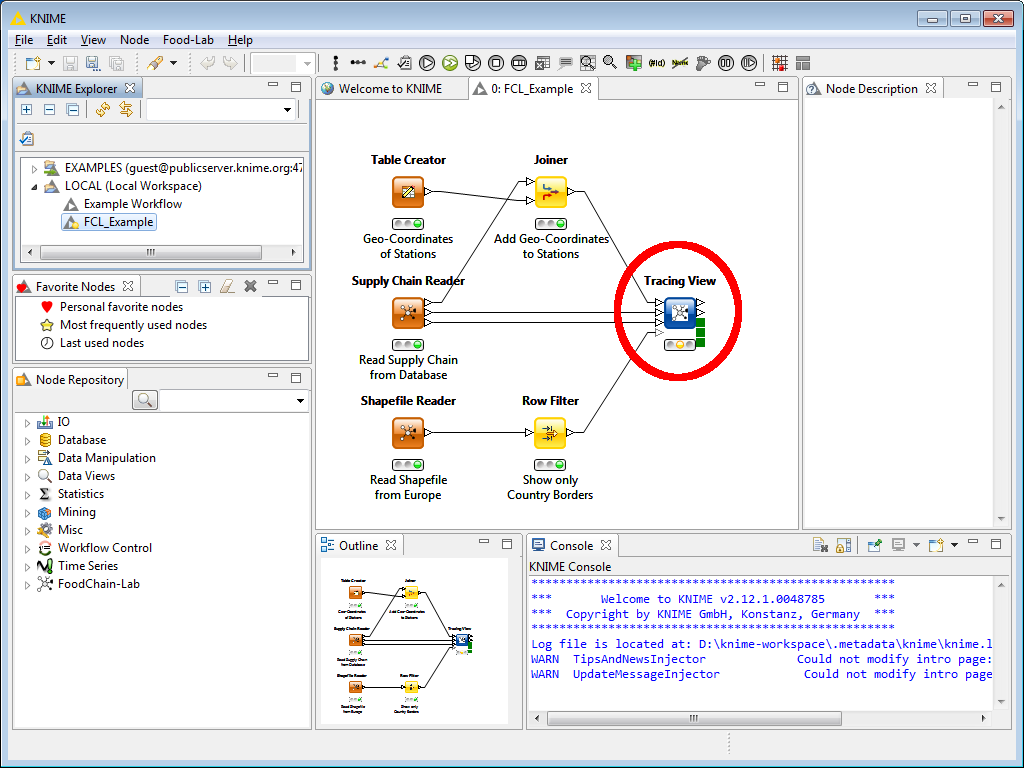
\includegraphics[height=0.6\textheight]{1.png}
	\end{center}
	\begin{itemize}
		\item Importieren sie den Example Workflow von \url{https://github.com/SiLeBAT/BfROpenLabResources/raw/master/GitHubPages/workflows/Example_Workflow.zip}.
		\item Öffnen sie den \textbf{Tracing View} per Doppelklick.
	\end{itemize}
\end{frame}

\section{2}
\begin{frame}
	\begin{center}
  		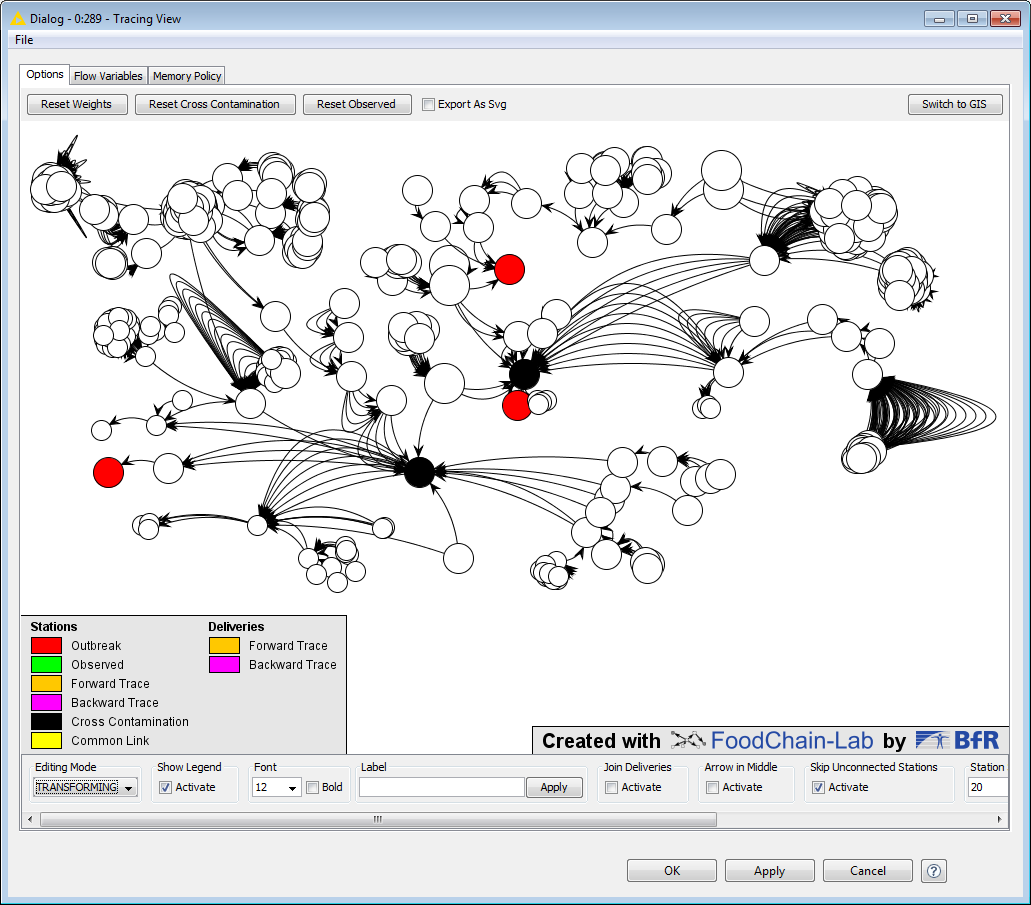
\includegraphics[height=0.6\textheight]{2.png}
	\end{center}
	\begin{itemize}
		\item Im Graphen sehen sie drei Ausbruchs-Stationen (rot) and zwei Stationen, an den Kreuzkontamination angenommen wird (schwarz).
		\item Die Größe jeder Station basiert auf ihrem "Score", welcher davon abhängt welche Ausbruchs-Stationen erreicht werden können.
	\end{itemize}
\end{frame}

\section{3}
\begin{frame}
	\begin{center}
  		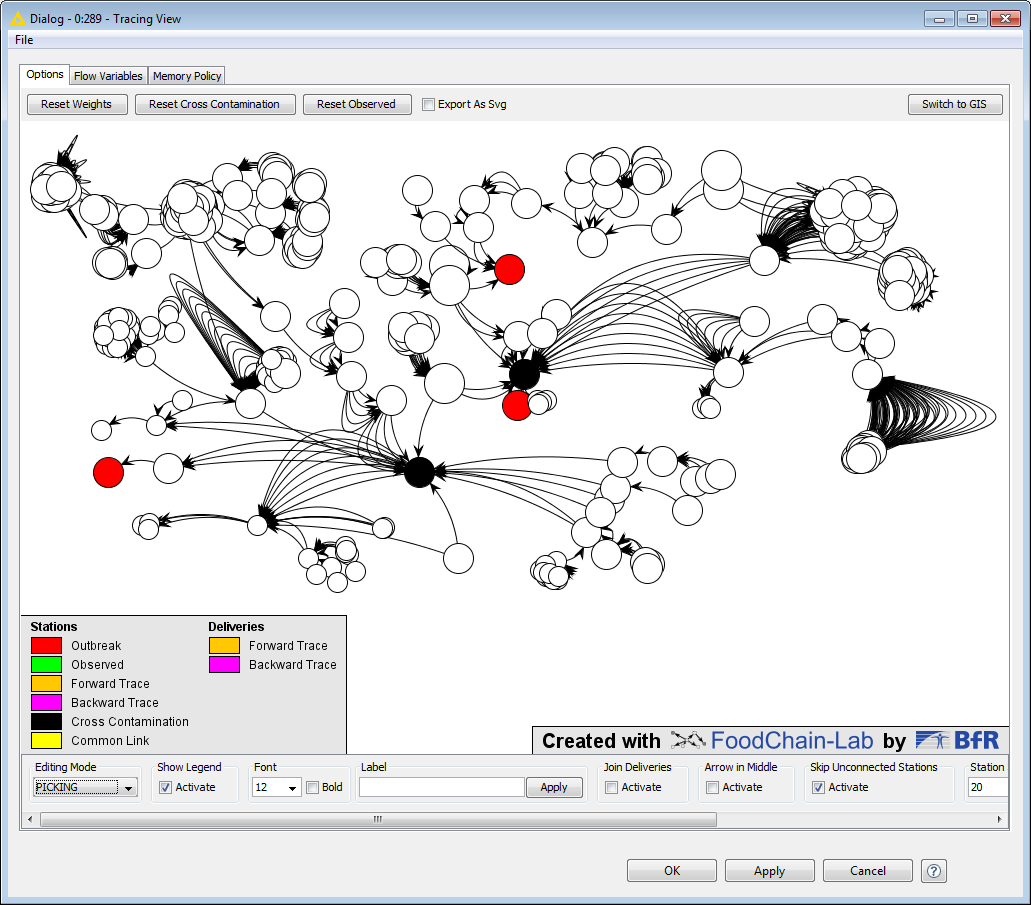
\includegraphics[height=0.6\textheight]{3.png}
	\end{center}
	\begin{itemize}
		\item Wir werden uns nun den Trace einer einzelnen Station im Detail anschauen.
		\item Wählen sie "PICKING" als \textbf{Editing Mode} und machen sie einen Doppelklick auf die Station im roten Kreis.
	\end{itemize}
\end{frame}

\section{4}
\begin{frame}
	\begin{center}
  		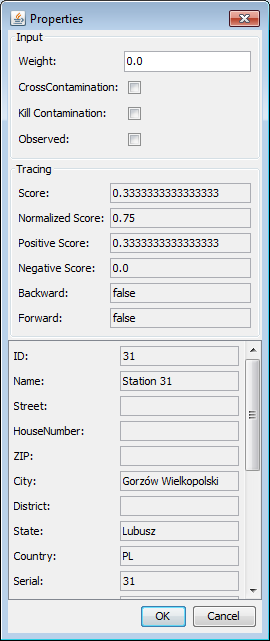
\includegraphics[height=0.6\textheight]{4.png}
	\end{center}
	\begin{itemize}
		\item Ein Dialog mit allen Attributen der ausgewählten Station erscheint.
		\item Im oberen Bereich können sie die Werte der Attribute "Weight", "CrossContamination" und "Observed" verändern.		
	\end{itemize}
\end{frame}

\section{5}
\begin{frame}
	\begin{center}
  		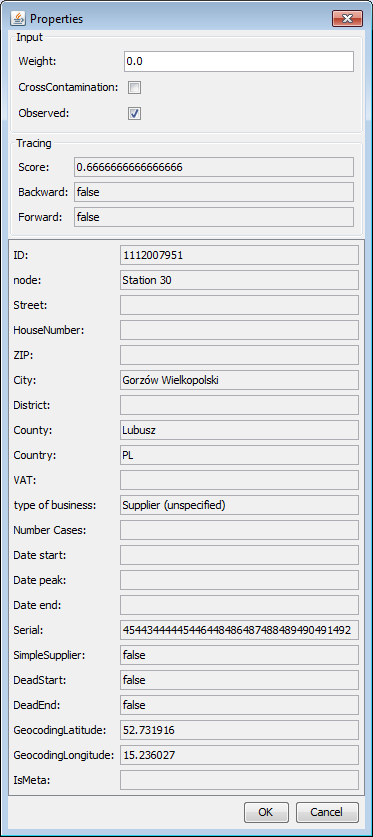
\includegraphics[height=0.6\textheight]{5.png}
	\end{center}
	\begin{itemize}
		\item Aktivieren sie \textbf{Observed} und drücken sie \textbf{OK}.
	\end{itemize}
\end{frame}

\section{6}
\begin{frame}
	\begin{center}
  		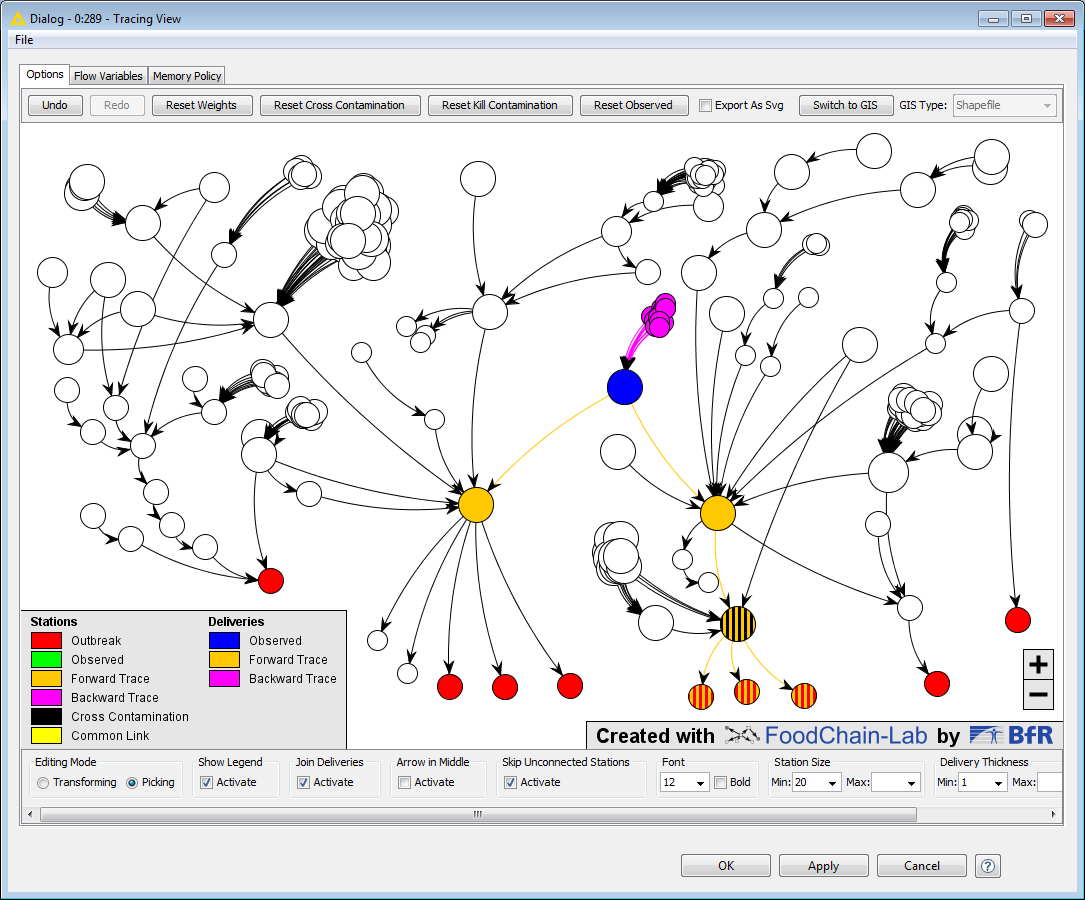
\includegraphics[height=0.6\textheight]{6.png}
	\end{center}
	\begin{itemize}
		\item Alle Stationen/Lieferungen vom Forward-Trace sind orange gefärbt and diejenigen vom Backward-Trace sind lila.
		\item Zwei der drei Ausbruchs-Stationen sind nun orange gestreift. Das bedeutet, dass sie auch auf dem Forward-Trace sind.
	\end{itemize}
\end{frame}

\section{7}
\begin{frame}
	\begin{center}
  		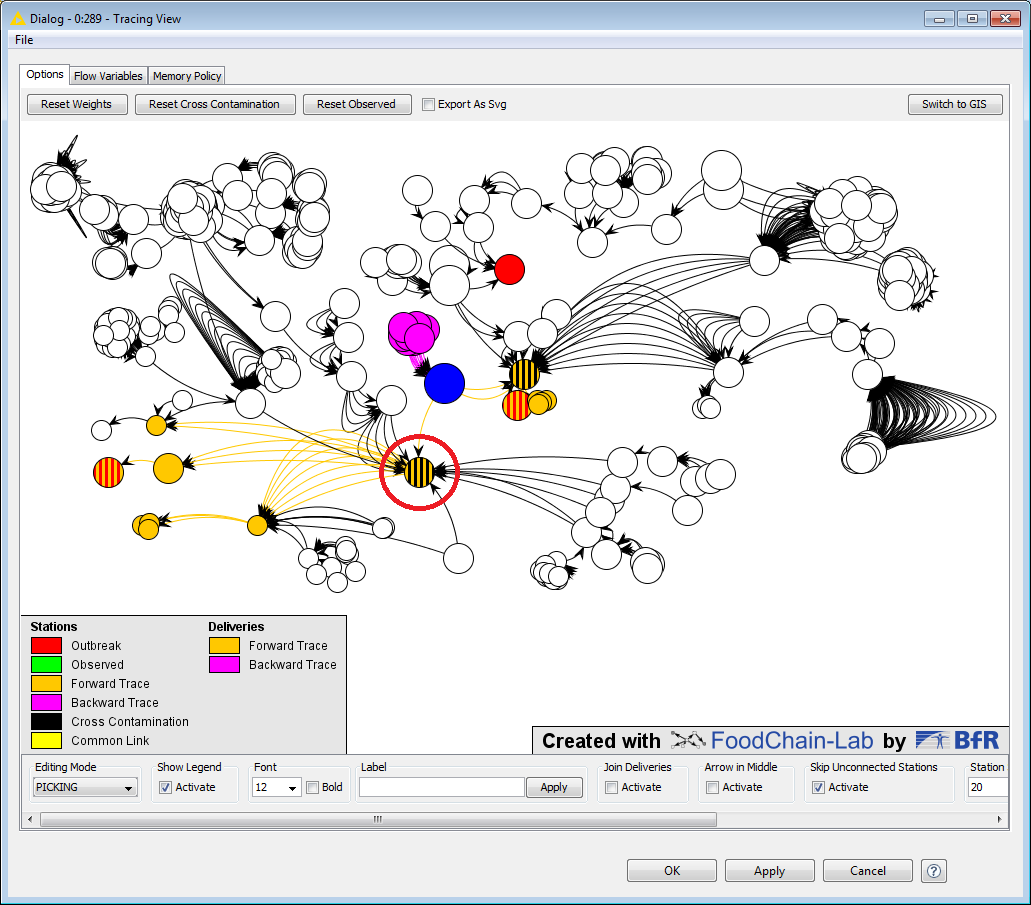
\includegraphics[height=0.6\textheight]{7.png}
	\end{center}
	\begin{itemize}
		\item Nun schauen wir was sich verändert, wenn wir die Kreuzkontamination der Station im roten Kreis deaktivieren.
		\item Machen sie einen Doppelklick auf die Station.
	\end{itemize}
\end{frame}

\section{8}
\begin{frame}
	\begin{center}
  		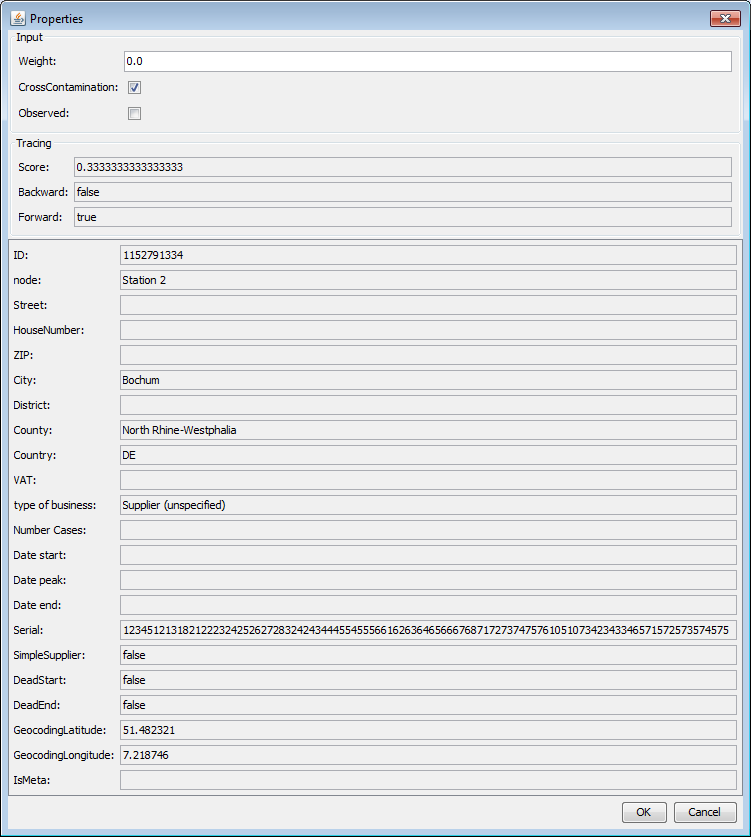
\includegraphics[height=0.6\textheight]{8.png}
	\end{center}
	\begin{itemize}
		\item Deaktivieren sie \textbf{CrossContamination} und drücken sie \textbf{OK}.
	\end{itemize}
\end{frame}

\section{9}
\begin{frame}
	\begin{center}
  		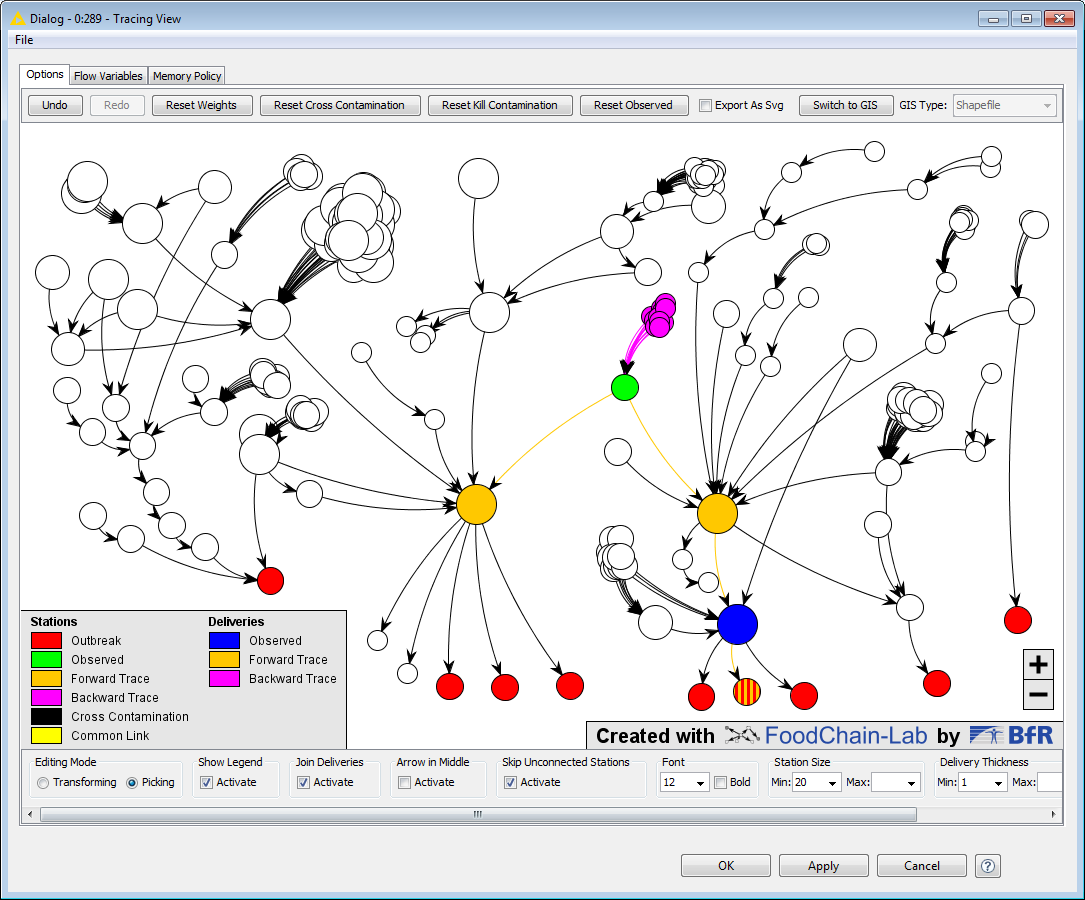
\includegraphics[height=0.6\textheight]{9.png}
	\end{center}
	\begin{itemize}
		\item Das Deaktivieren der Kreuzkontamination hat den Forward-Trace der beobachteten Station ("Observed") verändert.
		\item Nun kann die ganz linke Ausbruchs-Station nicht mehr erreicht werden.
	\end{itemize}
\end{frame}

\end{document}